De acuerdo con el montaje experimental descrito anteriormente,
se registraron valores de corriente que generaban un campo magnético suficiente
para corregir la deflexión inducida sobre el haz de electrones.
Estos valores se presentan en la \cref{tab:data}, donde los campos magnéticos
fueron calculados utilizando la \cref{eq:magnetic-field}, y la carga específica
del electrón fue obtenida mediante la \cref{eq:specific-charge}.

\begin{table}[htbp!]
	\centering
	\rowcolors{2}{white}{gray!25}
	\begin{tabular}{S[table-format=3.1(2)]|S[table-format=2.1(1)]
		|S[table-format=1.2(1)]|S[table-format=1.1(1)e2]}
	\toprule
	{\(U_a \, (\unit{V})\)} & {\(U_d \, (\unit{V})\)} & {\(I \, (\unit{A})\)} &
	{\(e/m \, (\unit{C \per kg})\)} \\
	\midrule
	390.0(1) & 36.5(1) & 0.06(1) & 7(2)e+11 \\
	390.0(1) & 45.5(1) & 0.06(1) & 1.0(3)e+12 \\
	390.0(1) & 63.5(1) & 0.09(1) & 9(1)e+11 \\
	445.6(1) & 39.0(1) & 0.06(1) & 7(2)e+11 \\
	445.6(1) & 50.6(1) & 0.03(1) & 4(2)e+12 \\
	445.6(1) & 70.7(1) & 0.11(1) & 6(1)e+11 \\
	523.0(1) & 43.4(1) & 0.05(1) & 1.0(4)e+12 \\
	523.0(1) & 58.0(1) & 0.08(1) & 7(2)e+11\\
	523.0(1) & 81.3(1) & 0.10(1) & 9(1)e+11\\
	\bottomrule
	\end{tabular}
	\caption{Valores para el campo magnetico y la carga especifica.}
	\label{tab:data}
\end{table}


Se observa una repetición de ciertos valores para la carga específica,
así como para la corriente en distintos valores de potencial.
Al promediar la carga específica,
se obtiene un valor de \(e / m \approx \qty{1.2(5)e+12}{C \per kg}\),
con una desviación estándar de \num{1.07}, lo que representa una incertidumbre
considerable.

El valor reportado en la literatura para la carga específica del electrón es
\(e / m = \qty{1.76e11}{C \per kg}\) \cite{nist-2024}, lo que implica un error
relativo porcentual del \qty{298}{\percent} utilizando el límite inferior del
intervalo de confianza, y del \qty{582}{\percent} si se toma el valor central
del intervalo.

Este margen de error, notablemente elevado, sugiere la existencia de errores
significativos en el montaje experimental o en el procesamiento de los datos.
Dado que se observaron valores repetidos de corriente, se realizó una
representación tridimensional del campo magnético \(B\) en función de \(U_a\) y
\(U_d\), como se ilustra en la \cref{fig:magnetic-field}.
Para obtener la superficie teórica de los valores esperados, se despejó el campo
magnético a partir de la \cref{eq:specific-charge}, empleando el valor de
referencia de la carga específica.

\begin{figure}[htbp!]
  \centering
  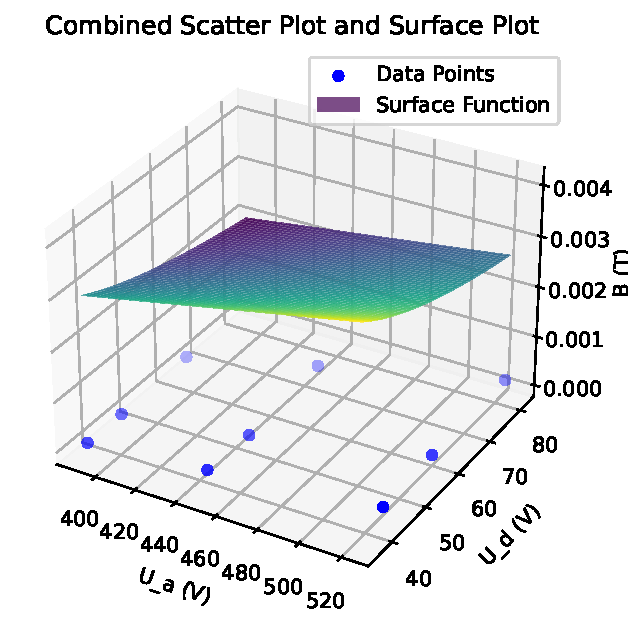
\includegraphics[width=0.8\linewidth]{./images/Magnetic_Field.pdf}
  \caption{Comparación entre el campo magnético obtenido y el esperado.}
  \label{fig:magnetic-field}
\end{figure}

Es evidente que los valores experimentales del campo magnético son inferiores en
casi un orden de magnitud con respecto a los valores teóricos esperados.
Esta discrepancia sustancial entre el campo magnético medido y el esperado
explica tanto el error en el orden de magnitud como la desviación en el valor de
la carga específica calculada.
